\documentclass{article}

%~~~~~~~~~ Document setup
\usepackage[english]{babel} % English formatting
\usepackage[utf8]{inputenc} % Standard encoding
\usepackage[a4paper,left=3cm,bottom=3cm]{geometry} % Page formatting
\usepackage{indentfirst} % Indents the first paragraph
\usepackage{amsmath} % Maths type package
\usepackage{bm} % Bold font maths
\usepackage{graphicx} % Advanced graphics package
\usepackage[export]{adjustbox} 
\usepackage{pdflscape} % Make pages landscape
\usepackage{fancyhdr} % Fancy headers
\usepackage[colorlinks=true,citecolor=blue,urlcolor=blue,linkcolor=black]{hyperref} % Link colours
\usepackage{natbib} % Bibliography
\usepackage{flafter} % Reference any 'float'
\usepackage[framemethod=tikz]{mdframed} % Box off stuff
\usepackage{color} % Colour support
\usepackage{wrapfig} % Text flowing around figures
\usepackage{lipsum} % Generates meaningless text
\usepackage{listings}
\usepackage{xcolor}
\definecolor{codegreen}{rgb}{0,0.6,0}
\definecolor{codegray}{rgb}{0.5,0.5,0.5}
\definecolor{codepurple}{rgb}{0.58,0,0.82}
\definecolor{backcolour}{rgb}{0.95,0.95,0.92}

\lstdefinestyle{mystyle}{
    backgroundcolor=\color{backcolour},   
    commentstyle=\color{codegreen},
    keywordstyle=\color{magenta},
    numberstyle=\tiny\color{codegray},
    stringstyle=\color{codepurple},
    basicstyle=\ttfamily\footnotesize,
    breakatwhitespace=false,         
    breaklines=true,                 
    captionpos=b,                    
    keepspaces=true,                 
    numbers=left,                    
    numbersep=5pt,                  
    showspaces=false,                
    showstringspaces=false,
    showtabs=false,                  
    tabsize=2
}
 
\lstset{style=mystyle}
\graphicspath{ {Images/} } % Folder for images 

%~~~~~~~~~ Multi-column setup
\usepackage{multicol} % Multi Column Environment
\setlength{\columnsep}{1cm}
\setlength{\columnseprule}{1pt}
\def\columnseprulecolor{\color{black}} % comment this to remove the line
\usepackage{float} % Lets you add images to multi-column environment

%~~~~~~~~~ Page setup
\pagestyle{fancy}
\fancyhf{}
\lhead{Sajid-Lulwa-Tuck}
\lfoot{Brushless Motor Controller}
\rhead{March 2020}
\rfoot{Page \thepage}
\renewcommand{\footrulewidth}{0.4pt}

%~~~~~~~~~ Title
\title{Brushless Motor Controller}
\author{Sajid Lulwa Louys}
\date{\today}

%~~~~~~~~~ Document start
\begin{document}

\begin{titlepage}
    \begin{center}
        \vspace*{1cm}
            
        \Huge
        \textbf{Embedded Systems}
            
        \vspace{0.5cm}
        \LARGE
        \textbf{Brushless Motor Controller}
            
        \vspace{1.5cm}
            
        \textbf{Team Name: Friends}\\ 
            
        \vfill
            
        Coursework 2 Report\\
       
            
        \vspace{0.8cm}
         
            
        \Large
        \textbf{Team Members:}\\
        Sajid Ali\\
        Tuck Hong 01336059\\
        Lulwa Alkhalifa 01351905 \\
            
    \end{center}
\end{titlepage}


\pagenumbering{gobble} % keep title page without a number
%\maketitle
\tableofcontents
\thispagestyle{empty} % remove page numbering for contents page
\clearpage

\pagenumbering{arabic} % start page numbers again
\setcounter{page}{1}

\section{Introduction}
\subsection{Brief}
In this report is summarised the implementation of a brushless motor controller which performs additional lower priority tasks in an embedded system.

\subsection{Specification}
\noindent The system was designed to meet the following design criteria:
 \begin{itemize}
	\item Motor will spin for defined number of rotations and stop without overshooting with a precision of \underline{0.5 rotations per number of rotations}.
	\item Motor will spin at a defined maximum angular velocity \underline{5-100 rotations per second}, with a precision of \underline{0.5 rotations per second}.
	\item Perform Bitcoin mining task and test \underline{5000 nonces per second}. Matching nonces will be sent back to the host.
	\item Motor will play a melody while it is spinning. The melody is a repeating sequence of notes in C4 octave with durations of \underline{0.125-1 seconds}.
\end{itemize}





\section{Motor Control Implementation}
\subsection{Position and Velocity Measurements}

I'm guessing this has probably changed since yesterday. I'm so sorry about that :(

\subsection{Velocity Control}

\noindent
Velocity was controlled using a proportional and integral term in the control equation.

\[ y_s = \left( k_p(s-v)+ k_i\int(s-v)dt\right)\textrm{sgn}(E_r)\]

\noindent
\(y_s\) is the speed controller output which is compared with the position controller output to determine the motor PWM. \(k_p\)and \(k_i\) are the tuning parameters, \(s\) is the maximum speed (set by the host and initialised at 100 rotations per second upon startup) , \(E_r\) is the position error, and \(v\) is the measured velocity. The integral term is implemented as follows:

\bigskip

\lstinputlisting[language=C++]{velocity1.cpp}


\bigskip

\noindent
Further processing is done to convert the controller output into a PWM duty cycle. The absolute value of \(y_s\) is considered and the value of lead is modified to take the direction of rotation into account.

\bigskip

\lstinputlisting[language=C++]{velocity2.cpp}

\bigskip

\noindent
Also a limit is applied so that the PWM duty cycle (\textbf{power}) does not exceed the maximum value of 1

\bigskip

\lstinputlisting[language=C++]{velocity3.cpp}

\bigskip

\subsection{Position Control}

\noindent
For position control both a proportional and differential term are used.

\[y_r = k_pE_r + k_d \frac{dE_r}{dt}\]

\(k_p\) and \(k_d\) are the tuning parameters, and \(E_r\) is the position error. This is calculated as shown below:

\bigskip
\lstinputlisting[language=C++]{position1.cpp}
\bigskip

\noindent
Combining velocity and position control is done by choosing the most conservative value and is implemented as follows:

\bigskip
\lstinputlisting[language=C++]{position2.cpp}
\bigskip

\noindent
A non-linearity is applied the distance error term to prevent oscillations at lower speeds.

\section{Tasks and Dependencies}
\subsection{Motor Control}

\noindent
Motor control is implemented in a high priority thread \textbf{motorCtrlT}. Within the main function responsible for motor control \textbf{motorCtrlFn}, the interrupt service routine \textbf{UpdateMotorPos} is attached to the photo-interrupter inputs, such that the motor PWM is updated whenever there is a change in any of the inputs.

\bigskip

\noindent
A ticker object is also created within \textbf{motorCrtlT} and the callback function \textbf{motorCtrlTick()} is attached, such that it runs every 100ms. The purpose of this interrupt is to set a signal using the RTOS function \textbf{Thread::signal\_set()} to \textbf{motorCtrlT}. This ensures that velocity is measured and the control output for power is updated every 100ms.

\bigskip
\lstinputlisting[language=C++]{motor1.cpp}
\bigskip

\noindent
Furthermore, when calculating velocity and distance error, the mutex \textbf{maxSpeed\_mutex }is used to protect the variable \textbf{maxSpeed} and the mutex \textbf{targetPosition\_mutex} is used to protect the variable \textbf{targetPosition} from simulataneous access. This is important because the decode command thread also needs to write to these variables when speed and position commands are received from the host. An example of this is shown below.

\bigskip
\lstinputlisting[language=C++]{motor2.cpp}
\bigskip

\subsection{Melody}

\noindent
By modulating the PWM period and hence the drive current, the motor effectively behaves like a tune generator. A separate thread \textbf{TuneThread} is responsible for changing the PWM period based on the notes present in melody commands given by the user. The notes that are allowed belong to the C4 octave, in other words, frequencies 261.63 Hz (C4) up to 493.88 Hz (B4).   

\bigskip

\noindent
First, a map containing all the allowed notes and their corresponding PWM periods is initialised. Note that the PWM periods (in $\mu$s) are calculated using $\frac{1000000}{frequency}$. 

\bigskip

\lstinputlisting[language=C++]{melody1.cpp}

\bigskip

\noindent
In an infinite loop, the thread repeats the following steps where \textbf{tonesQ} is a queue containing the notes and durations that need to be played. 

\bigskip

\lstinputlisting[language=C++]{melody2.cpp}

\bigskip

\noindent
Since \textbf{tonesQ} is a shared data structure also accessed by \textbf{TerminalListenerThread}, the popping and pushing actions are protected with a mutex. Note that after popping a tone from \textbf{tonesQ} the same tone is immediately pushed back, as the specification requires the motor to play a given melody on loop. 

\bigskip

\noindent
Following the regex for melody commands where the last entry in the command is an integer corresponding to the duration of the note (number of eighths of a second), the exact duration in milliseconds is obtained in line 8. Note that \textbf{(int)'0'} represents the offset value for numerical ASCII characters such that when subtracted from \textbf{(int)duration}, duration (which is a \textbf{char}) is effectively ``converted" into an \textbf{int}. 

\bigskip

\noindent
After setting the new PWM period using \textbf{tone} and \textbf{tonefreqmap} initialised previously, the thread is then put to sleep using \textbf{ThisThread::sleep\_for(interval)} so that a given note will last for the specified amount of time before the loop continues with the next note to be played. This solves the issue of blocking other threads from running (e.g. the bitcoin thread which will result in the thread failing to meet 5000 nonces per second) when \textbf{wait} is used instead.   

\bigskip

\noindent
This task is dependent on a non-empty \textbf{tonesQ}. This dependency is released by \textbf{TerminalListenerThread} when a melody command is received from the user. 

\subsection{Decoding Messages}

\noindent The system receives commands from a host over a serial interface at 9600bps and follows the given syntax specifications:

 \begin{itemize}
	\item Each command ends with a carriage return character.
	\item The syntax for rotation commands is the regular expression R-?\textbackslash{}d\{1,4\}(\textbackslash{}.\textbackslash{}d)?
	\item The syntax for maximum speed commands is the regular expression V\textbackslash d \{1,3\}(\textbackslash{}.\textbackslash{}d)?
	\item The syntax for setting the bitcoin key is the regular expression K[0-9a-fA-F]\{16\}
	\item Matching bitcoin nonces should be sent to the host with a message matching the regular expression N[0-9a-fA-F]\{16\}
	\item The syntax for melody commands is the regular expression T([A-G][\#\textasciicircum{}]?[1-8])\{1,16\} (where \# and \textasciicircum{}are characters)
	
\end{itemize}

\noindent
An interrupt service routine \textbf{serialISR} receives each incoming byte from the serial port and places it into a queue. This is done by using the method \textbf{uint8\_t RawSerial::getc()} to retrieve a byte from the serial port and the method \textbf{Mail::put()} to put a \textbf{Mail} message in a \textbf{mail\_box} queue.
\bigskip

\noindent
Decoding messages is implemented in \textbf{TerminaListenerThread} as a normal priority thread. \textbf{serialISR} is attached to serial port events, and in an infinite loop the method \textbf{Mail::get()} is used to wait for new characters. Upon receiving a return carriage character from mail, the command message is passed to functions that try to match it with the expected syntax. The command message is then placed in another \textbf{mail\_box} to be communicated to the host via serial.

\bigskip
\lstinputlisting[language=C++]{decode1.cpp}   
\bigskip       

\noindent
The method used detemine if the command message is valid varies for the different commands.The standard C++ regular expressions library is used to decode speed and position commands. The function \textbf{sscanf} is used to decode the new key command, and melody commands are decoded by iterating through the message string as shown below.

\bigskip
\lstinputlisting[language=C++]{decode2.cpp}  
\bigskip
If the message received from the serial port matches any of the expected commands, then the relevant changes are made to implement the command and a \textbf{Mail} message to confirm receiving a command is put into a \textbf{mail\_box} and communicated to the host via serial. 
\bigskip

In \textbf{decodeSpeedCommand}, for example, the new maximum speed is written into a global variable \textbf{maxSpeed} where it will be read by the motor control thread. This variable is protected by a mutex \textbf{maxSpeed\_mutex} to prevent simultaneous access.


\subsection{Outputting Messages}

\subsection{Bitcoin Mining}

\noindent
The bitcoin mining task is implemented in \textbf{BitcoinThread} as a low priority thread. The task is to look for matching nonces such that when combined with a key provided by the user and the 48 bytes of constant payload, will produce a SHA-256 hash that begins with 16 zeros. This is done by simply initialising the nonce to 0 and incrementing by one on each attempt. 

\bigskip

\noindent
In order to regulate the mining task so that it satisfies the throughput specification of exactly 5000 nonces per second, the \textbf{Ticker} class is used to set up a timer interrupt that sends a signal to \textbf{BitcoinThread} every second. Every time the thread is released by the signal (which happens once per second), 5000 nonces are tested. The specification also requires the thread to send matching nonces back to the host. This is done by putting a \textbf{Mail} message pointer of type \textbf{BITCOIN\_NONCE} in the \textbf{mail\_box} queue. 

\bigskip

\lstinputlisting[language=C++]{bitcoin1.cpp}

\bigskip

\noindent
A dependency this task has is the semaphore-like signal from the timer interrupt. This dependency is released once per second (by the timer interrupt). Note that a mutex is used here as \textbf{newKey} is a shared variable that is also accessed by \textbf{TerminalListenerThread} when a new bitcoin key is set by the user. 


\subsection{Dependency Graph}

\begin{figure}[H]
\begin{center}
%\fbox{\rule{0pt}{1in} \rule{0.8\linewidth}{0pt}}
   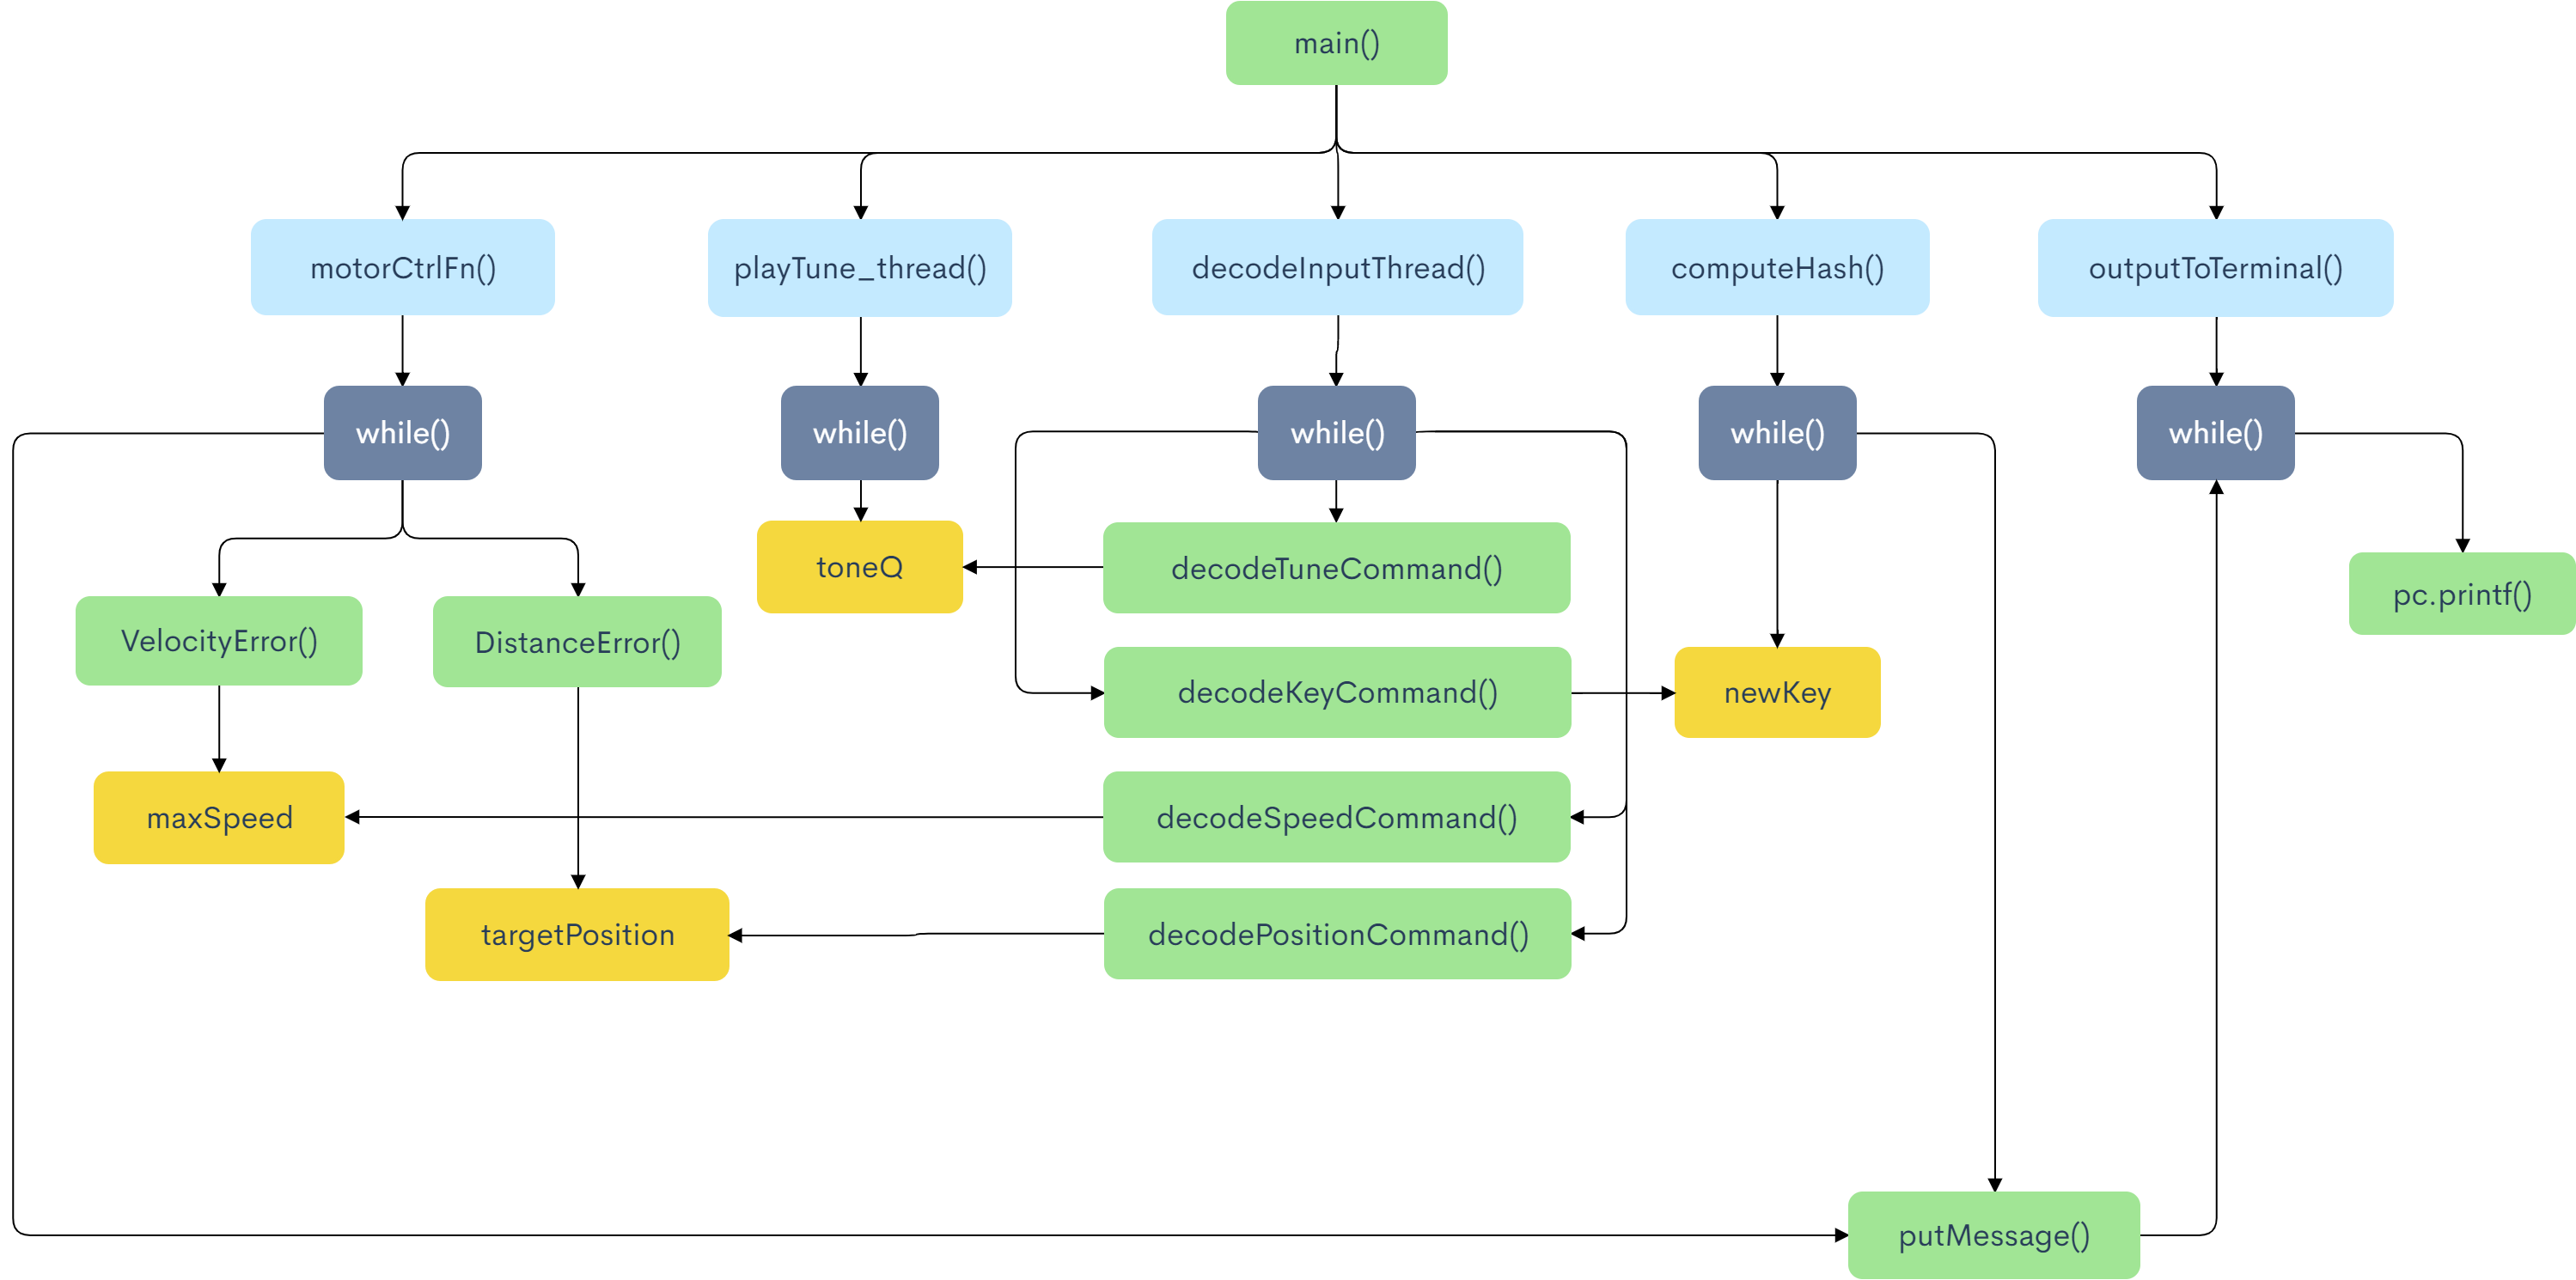
\includegraphics[width=0.9\linewidth]{dependency.png}
\end{center}
   \caption{Dependency flow chart.}
\label{fig:long}
\label{fig:onecol}
\end{figure}

\section{Timings and CPU Utilisation}
\subsection{Methodology}

\noindent
The CPU usage of each task running in the micro-controller was indirectly observed by pulling one of the digital I/O pins high and low to show when a task was executing. Measuring the time the between pulses and the duration of each pulse would tell us the initiation interval and execution time of each task.

We used a USB oscilloscope to take the measurements. An example of a trace we obtained is shown below.

\begin{figure}[H]
\begin{center}
%\fbox{\rule{0pt}{1in} \rule{0.8\linewidth}{0pt}}
   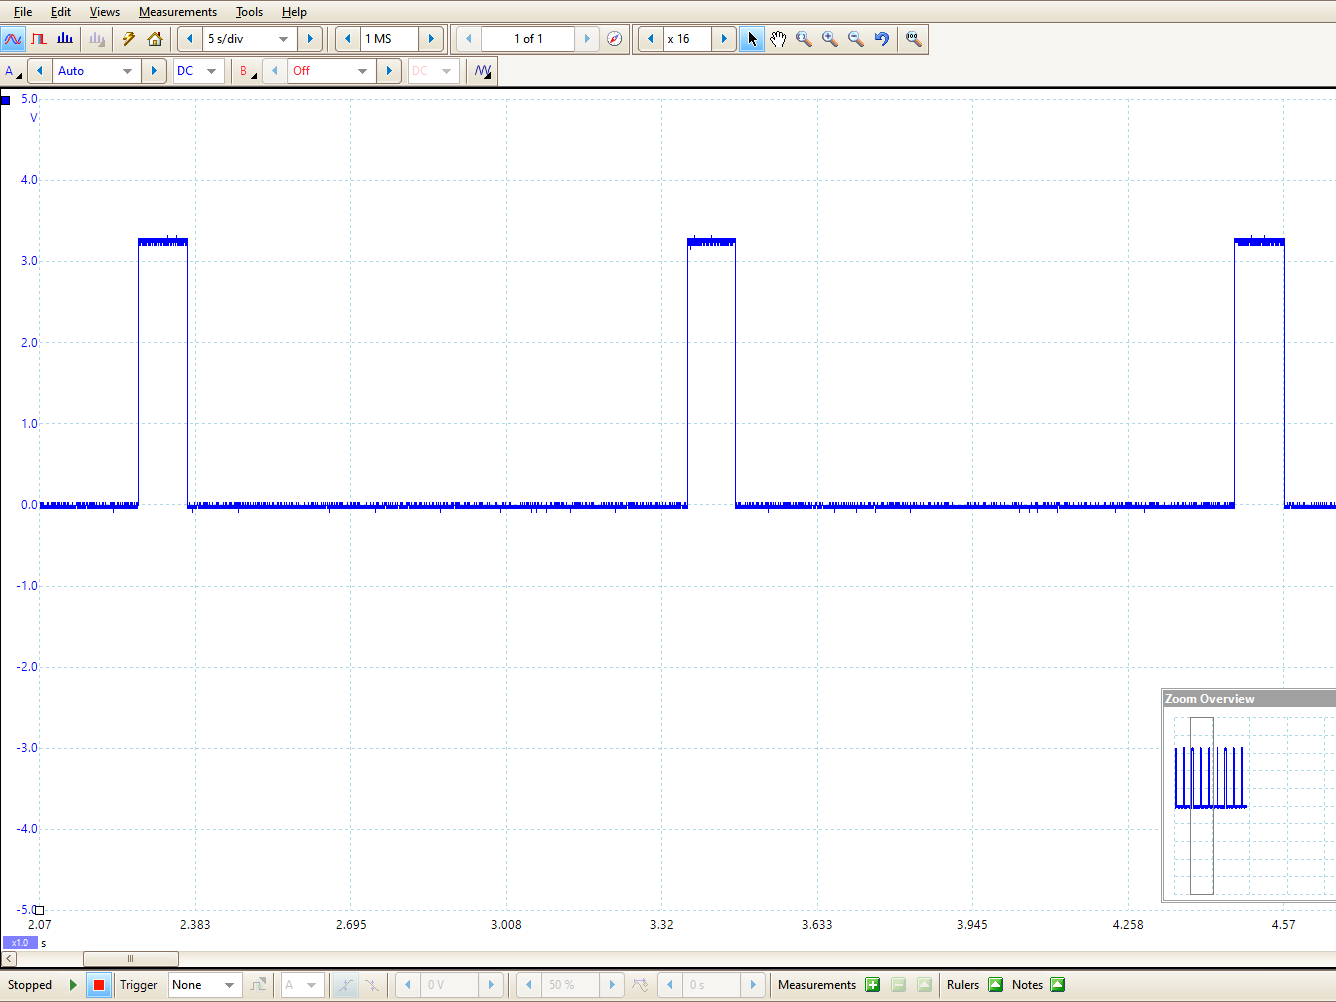
\includegraphics[width=0.9\linewidth]{ScopeOutput.png}
\end{center}
   \caption{Picoscope pulse trigger.}
\label{fig:long}
\label{fig:onecol}
\end{figure}


\subsection{Measure Results}

\begin{table}[ht]
\centering                      % used for centering table
\begin{tabular}{c c c c}        % centered columns (4 columns)
Task & Initiation Interval (t) & Execution Time (T) & CPU Utilization (U) \\ [0.5ex]   % inserts table %heading
\hline                          % inserts 1 horizontal line
ISR & 1.28ms & 5.0us & 0.40\% \\           % table contents
Output & 1.0s & 101ms & 10.11\% \\                         
Motor Control & 100ms & 75us  & 0.08\% \\
Decode & - & 53us & - \\
BitCoin Mining & 1.0s & 868ms & 86.8\% \\
Melody & 0.125s & 1.0us & ~0\% \\[1ex]     % [1ex] adds vertical space
\end{tabular}
\caption{Task timing and resource utilization.} 
\label{table:nonlin}            % is used to refer this table in the text
\end{table}


\subsection{Critical Instant Analysis of the Rate Monotonic Scheduler}

\noindent
By assuming the worst case scenario in terms of resource usage, we can test to see if our design will always meet the specifications.
To test this we will calculate the CPU time used up by every thread within a single second. If we are able to execute all necessary tasks within this time frame, then we can be confident in our design.

\bigskip

\noindent
We start by assuming that the motor is running at full speed (i.e. 100 rps) and that we are printing to the terminal every second.

\bigskip

\noindent
Using the table above, this yields 3.6ms and 0.75ms of CPU time for the motor interrupt and motor control threads respectively.
The final three threads, printing, bitcoin mining, and playing a melody had fixed times and therefore can be added directly.

\bigskip

\noindent
The results are summarised in the figure below. As you can see, after all the tasks are done executing there is minimum surplus of 30ms which could be used to decoding messages from the user.


\begin{figure}[H]
\begin{center}
%\fbox{\rule{0pt}{1in} \rule{0.8\linewidth}{0pt}}
   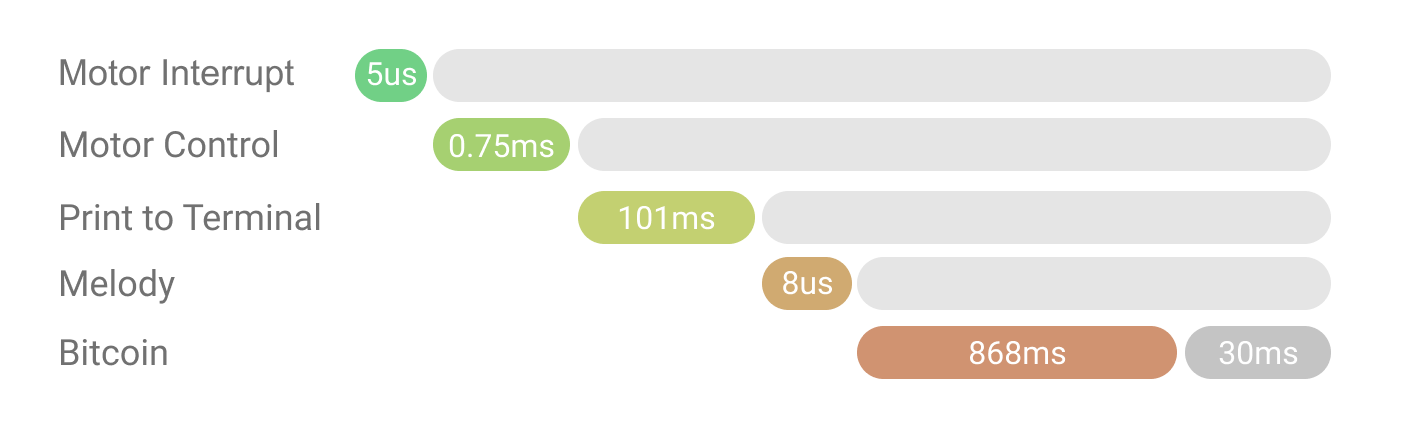
\includegraphics[width=0.9\linewidth]{scheduler.png}
\end{center}
   \caption{Worst case scenario scheduler.}
\label{fig:long}
\label{fig:onecol}
\end{figure}







\section{Citing and referencing}

\subsection{Referencing figures and equations}
 Expression $4\times 3=G\times x$ naturally follows from Eq \ref{eq:lovely formula}, and both of these things have a lot to do with Fig \ref{fig:frog in multicol}.
 
 \subsection{Citing a paper}
This statement has a citation at the end of it \cite{toadetal1958}, and this one has two \cite{toadetal1958, squeaker1982}. A citation with parenthesis is sure to follow \citep{siddiqi2004interspecific}.

 


%~~~~~~~~~ Bibliography
\bibliographystyle{abbrvnat}
\setcitestyle{authoryear}
\bibliography{bib}

\end{document}